%-----------------------------------------------------------------------
% Beginning of ofj-template.tex
%-----------------------------------------------------------------------
%
%     This is a topmatter template file for OpenFOAM Journal with LaTeX.
%
%     Templates for various common text, math and figure elements are
%     given following the \end{document} line.
%     This file is based on the template provided by AMS.
%
%%%%%%%%%%%%%%%%%%%%%%%%%%%%%%%%%%%%%%%%%%%%%%%%%%%%%%%%%%%%%%%%%%%%%%%%

%-----------------------------------------------------------------------
%      Copyright notice
%-----------------------------------------------------------------------
%
%      Authors of papers published  in the OpenFOAM journal retain 
%      copyright and release their work under the 
%      Creative Commons Attribution-ShareAlike 4.0 International License.
%      https://creativecommons.org/licenses/by-sa/4.0/
%      Any code snippets included in the manuscript as well as submitted 
%      source code as supplementary material are subject to 
%      the GNU General Public Licence. 
%      http://www.gnu.org/licenses/gpl-3.0.html
%      Any usage of the name OpenFOAM as well as the logo is being done 
%      with the full involvement of OpenCFD, trademark holder of 
%      OpenFOAM.
%
%-----------------------------------------------------------------------

%     Remove any commented or uncommented macros you do not use.

\documentclass[e-only,10pt,reqno]{ofj}

%     OpenFOAM-specific tensor and finite-volume notation packages
\usepackage{tensorNotation}
\usepackage{finiteVolumeNotation}

\usepackage{color}
\usepackage[dvipsnames,svgnames,x11names]{xcolor}
\usepackage{comment}
\newcommand{\comment}[1]{}  %comment not showed

% Pick one of the following
\usepackage[markup=underlined]{changes} % Show changes
%\usepackage[final]{changes} % Final version

% In addition, comment the following line to hide the comment sections
\includecomment{comment}

% Define note (same as used in OFW bye-laws)
\newcommand{\note}[2][]{\added[#1,remark={#2}]{}}

% Define note colour by author
% If you would like to add notes, please add a line with your name here and a
% unique colour
\definechangesauthor[color=NavyBlue]{HN} %Håkan Nilsson
\definechangesauthor[color=Green]{PC} %Philip Cardiff
% \definechangesauthor[color=Bittersweet]{JS} % John Smith


%     Update the information is not the copyright
%     holder.
\copyrightinfo{2020}{OpenFOAM$^{\textregistered}$ Journal}
\numberwithin{equation}{section}
\newcommand{\OF}[0]{OpenFOAM\textsuperscript{\textregistered} }

\OpenFOAMversion{\OF v19xx}
\Repository{https://github.com/xxx}
\DOI{00.1000/xxx} %leave for submission



\begin{document}

% These notes are taken from the OFW16 Bye-Laws
\begin{comment}

%\begin{comment}
\section*{The actual document starts on next page. Some instructions:}

\section*{How to track changes}
\begin{itemize}
    \item Add your initials by \verb+\definechangesauthor+ above \verb+\begin{document}+.\\Pick your favourite color: \verb+https://en.wikibooks.org/wiki/LaTeX/Colors+
    \item This is how you \added[id=HN]{add} text:\\\verb+\added[id=HN]{add}+
    \item This is how you \added[id=HN, remark={comment}]{add (with comment)} text: \\\verb+\added[id=HN, remark={comment}]{add (with comment)}+
    \item This is how you \deleted[id=HN]{delete} text:\\\verb+\deleted[id=HN]{delete}+
    \item This is how you \deleted[id=HN, remark={comment}]{delete (with comment)} text:\\\verb+\deleted[id=HN, remark={comment}]{delete (with comment)}+
    \item This is how you make a note \note[id=HN]{A note}:\\\verb+\note[id=HN]{A note}+
    \item This is how you \replaced[id=HN]{replace}{relapce} text:\\\verb+\replaced[id=HN]{relapce}{replace}+
    \item This is how you \replaced[id=HN, remark={mis-spelled}]{replace (with comment)}{relapce (wthi coment)} text:\\\verb+\replaced[id=HN, remark={mis-spelled}]{relapse}{replace}+
    \item All markups can be removed by changing the header to \verb+\usepackage[final]{changes}+ later.
\end{itemize}

\newpage

\end{comment}


%    Abstract is required.
\begin{abstract}
This is the place for an abstract.
\end{abstract}

%    \title[short text for running head]{full title}
\title[\OF Journal publication]{\OF Journal publication}

%    Only \author and \address are required; other information is
%    optional.  Remove any unused author tags.

%    author one information
%    \author[short version for running head]{name for top of paper}
\author{Author1}
\address{Address1}
\curraddr{}
\email{Emailaddress1}
\thanks{}

%    author two information
\author{Author2}
\address{Address2}
\curraddr{}
\email{Emailaddress2}
\thanks{}


\date{xx.xx.202x}

\dedicatory{}


\maketitle

\section{Introduction}

This is the place for introduction.

\subsection{Subsection}

\begin{comment}
TEST TEST TES
\end{comment}


Example text: 

We shall consider the specific transport property $\Q$ and note that its spatial and temporal variation is governed by a second-order partical differential equation (PDE), viz.\
\begin{align}
    \ddt{}(\rho \Q) + \div(\rho \Q \U) - \Gamma_{\Q}\laplacian\Q - S_\Q(\Q) = 0.
    \label{eq:genTransEq}
\end{align}
Herein, $\Q=\Q(\xt)$ is an arbitrary general intensive physical quantitity, e.g., a fluid property (scalar or tensor of any rank). Thus, \eqref{eq:genTransEq} is often referred to as generic transport equation.

\OF (Open Field Operation And Manipulation) is a flexible and mature C++ Class Library for Computational Continuum Mechanics (CCM) and Multiphysics. Its Object-Oriented-Programming (OOP) paradigm enables to \emph{mimic data types and basic operations} of CCM using top-level syntax as close as possible to the conventional mathematical notation \emph{for tensors and partial differential equations}:
\begin{lstlisting}[emph={ddt,div,laplacian}]
solve
(
  fvm::ddt(rho,Phi)
  + fvm::div(phi, Phi)
  - fvm::laplacian(Gamma, Phi)
 ==
  Sphi
);
\end{lstlisting}
Beside providing OpenFOAM code itself, spatial and temporal discretisation of Eq.\ \ref{eq:genTransEq} can be also described in a precise and concise manner using the finite-volume notation\, \cite{Rusche2002} - see Tab.\ \ref{tab:FiniteVolumeNotation}.

\begin{table}
	\caption{Finite Volume Notation}
	\label{tab:FiniteVolumeNotation}
	\centering
		\begin{tabular}{p{0.3\textwidth}p{0.3\textwidth}}
		  \toprule
			  \multicolumn{2}{l}{implicit differential operators}\\
		  \midrule
			  rate of change     & $\fvmddt{\rho\q}$ \\%time derivative
			  convection term    & $\fvmdiv{F}{\q}{S}{\genFactor}$ \\
			  diffusion term     & $\fvmlaplacian{\Gamma}{\q}$ \\
			  linear part of source term & $\fvmSp{S_p}{\q}$ \\
			\hline
			  \multicolumn{2}{l}{explicit differential operators}\\
			\hline
			  temporal term      & $\fvcddt{\rho\q}$ \\
			  divergence term    & $\fvcdiv{\rho\U}{\q}{S}{\genFactor}$ \\
			  laplacian term     & $\fvclaplacian{\Gamma}{\q}$ \\
			  constant part of source term & $S_u$\\
		  \bottomrule
		\end{tabular}
\end{table}

\section{Theoretical backgroud}

Text in this section. Here is an examplary figure \ref{fig:example}.

%    Figure insertion; default placement is top; if the figure occupies
%    more than 75% of a page, the [p] option should be specified.
\begin{figure}
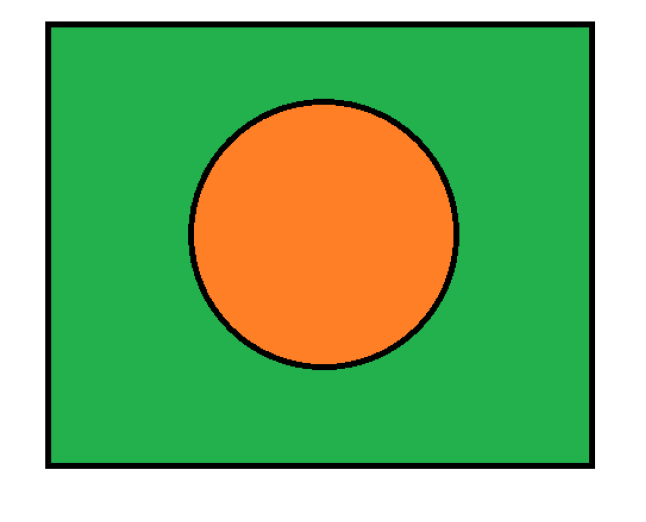
\includegraphics[width=0.5\textwidth]{example.png}
\caption{Examplary figure}
\label{fig:example}
\end{figure}


\section{Conclusion}

This is a conclusion.

%    Bibliographies can be prepared with BibTeX using IEEEtran style,
\bibliographystyle{IEEEtran}%do not change

%    Insert the bibliography data here.
\begin{thebibliography}{1}

\bibitem{Rusche2002}
H.~Rusche.
\newblock {\em {Computational Fluid Dynamics of Dispersed Two-Phase Flows at
  High Phase Fractions}}.
\newblock PhD thesis, {Imperial College of Science, Technology \& Medicine
  London}, 2002.

\end{thebibliography}


\end{document}

%%%%%%%%%%%%%%%%%%%%%%%%%%%%%%%%%%%%%%%%%%%%%%%%%%%%%%%%%%%%%%%%%%%%%%%%

%    Templates for common elements of a journal article; 

%    Section headings
\section{}
\subsection{}

%    Ordinary theorem and proof
\begin{theorem}[Optional addition to theorem head]
% text of theorem
\end{theorem}

\begin{proof}[Optional replacement proof heading]
% text of proof
\end{proof}

%    Figure insertion; default placement is top; if the figure occupies
%    more than 75% of a page, the [p] option should be specified.
\begin{figure}
\includegraphics{filename}
\caption{text of caption}
\label{}
\end{figure}

% Numbered equation
\begin{equation}
\end{equation}

% Unnumbered equation
\begin{equation*}
\end{equation*}

% Aligned equations
\begin{align}
  &  \\
  &
\end{align}

%-----------------------------------------------------------------------
% End of ofj-template.tex
%-----------------------------------------------------------------------
